%%%%%%%%%%%%%%%%%%%%%%%%%%%%%%%%%%%%%%%%%%%%%%%%%%%%%%%%%%%%%%%%%%%%%%%%%%%%%
%
%  System        : 
%  Module        : 
%  Object Name   : $RCSfile$
%  Revision      : $Revision$
%  Date          : $Date$
%  Author        : $Author$
%  Created By    : Robert Heller
%  Created       : Mon Jul 15 17:33:37 2019
%  Last Modified : <200211.1401>
%
%  Description 
%
%  Notes
%
%  History
% 
%%%%%%%%%%%%%%%%%%%%%%%%%%%%%%%%%%%%%%%%%%%%%%%%%%%%%%%%%%%%%%%%%%%%%%%%%%%%%
%
%    Copyright (C) 2019  Robert Heller D/B/A Deepwoods Software
%			51 Locke Hill Road
%			Wendell, MA 01379-9728
%
%    This program is free software; you can redistribute it and/or modify
%    it under the terms of the GNU General Public License as published by
%    the Free Software Foundation; either version 2 of the License, or
%    (at your option) any later version.
%
%    This program is distributed in the hope that it will be useful,
%    but WITHOUT ANY WARRANTY; without even the implied warranty of
%    MERCHANTABILITY or FITNESS FOR A PARTICULAR PURPOSE.  See the
%    GNU General Public License for more details.
%
%    You should have received a copy of the GNU General Public License
%    along with this program; if not, write to the Free Software
%    Foundation, Inc., 675 Mass Ave, Cambridge, MA 02139, USA.
%
% 
%
%%%%%%%%%%%%%%%%%%%%%%%%%%%%%%%%%%%%%%%%%%%%%%%%%%%%%%%%%%%%%%%%%%%%%%%%%%%%%

\chapter{QuadSMCSenseCape: Quad Motor Control and Sense Cape}


This is a circuit board to for an add-on board for a Beagle Bone Black that
will control four stall-motor turnout motors for a model railroad. It also has
sense logic to return the state of the turnouts, using one pole of the DPDT
contacts in the stall-motor (typical of Tortoise stall-motors).

The circuit board uses a pair of 46 pin header sockets to connect to the 46pin
headers on the Beagle Bone Black and can use a stack-through header to allow
additional boards to be stacked on top of it.

\section{GPIO Pins Used and stacking restrictions.}

This board uses eight GPIO pins:

\begin{description}
\item[GPIO 0.07, P9-42] Motor Select 1: select the position of stall motor 
1. 
\item[GPIO 1.6, P8-3] Motor Select 2: select the position of stall motor 
2. 
\item[GPIO 1.28, P9-12] Point Sense 1: return the state of the points for 
stall motor 1. 
\item[GPIO 1.7, P8-4] Point Sense 2: return the state of the points for 
stall motor 2. 
\item[GPIO 1.16, P9-15] Motor Select 3: select the position of stall motor 
3. 
\item[GPIO 1.17, P9-23] Motor Select 4: select the position of stall motor 
4. 
\item[GPIO 3.21, P9-25] Point Sense 3: return the state of the points for 
stall motor 3. 
\item[GPIO 3.19, P9-27] Point Sense 4: return the state of the points for 
stall motor 4. 
\end{description}

Each of the motor drive circuits is through a TC4428, which can drive up to
1.5A, which is way more needed to drive typical stall motor. It is enough to
drive a pair of stall motors, wired in parallel as would be the case for a
cross over. 

Because this board is hardwired to use eight specific GPIO pins it is not 
possible to use two or more of these boards on given Raspberry Pi.

\section{Circuit Description}

\begin{figure}[hbpt]\begin{centering}%
\includegraphics[width=5in]{QuadSMCSenseCape-1.pdf}
\caption{Circuit Diagram of the QuadSMCSenseCape, Sheet 1}
\end{centering}\end{figure}
\begin{figure}[hbpt]\begin{centering}%
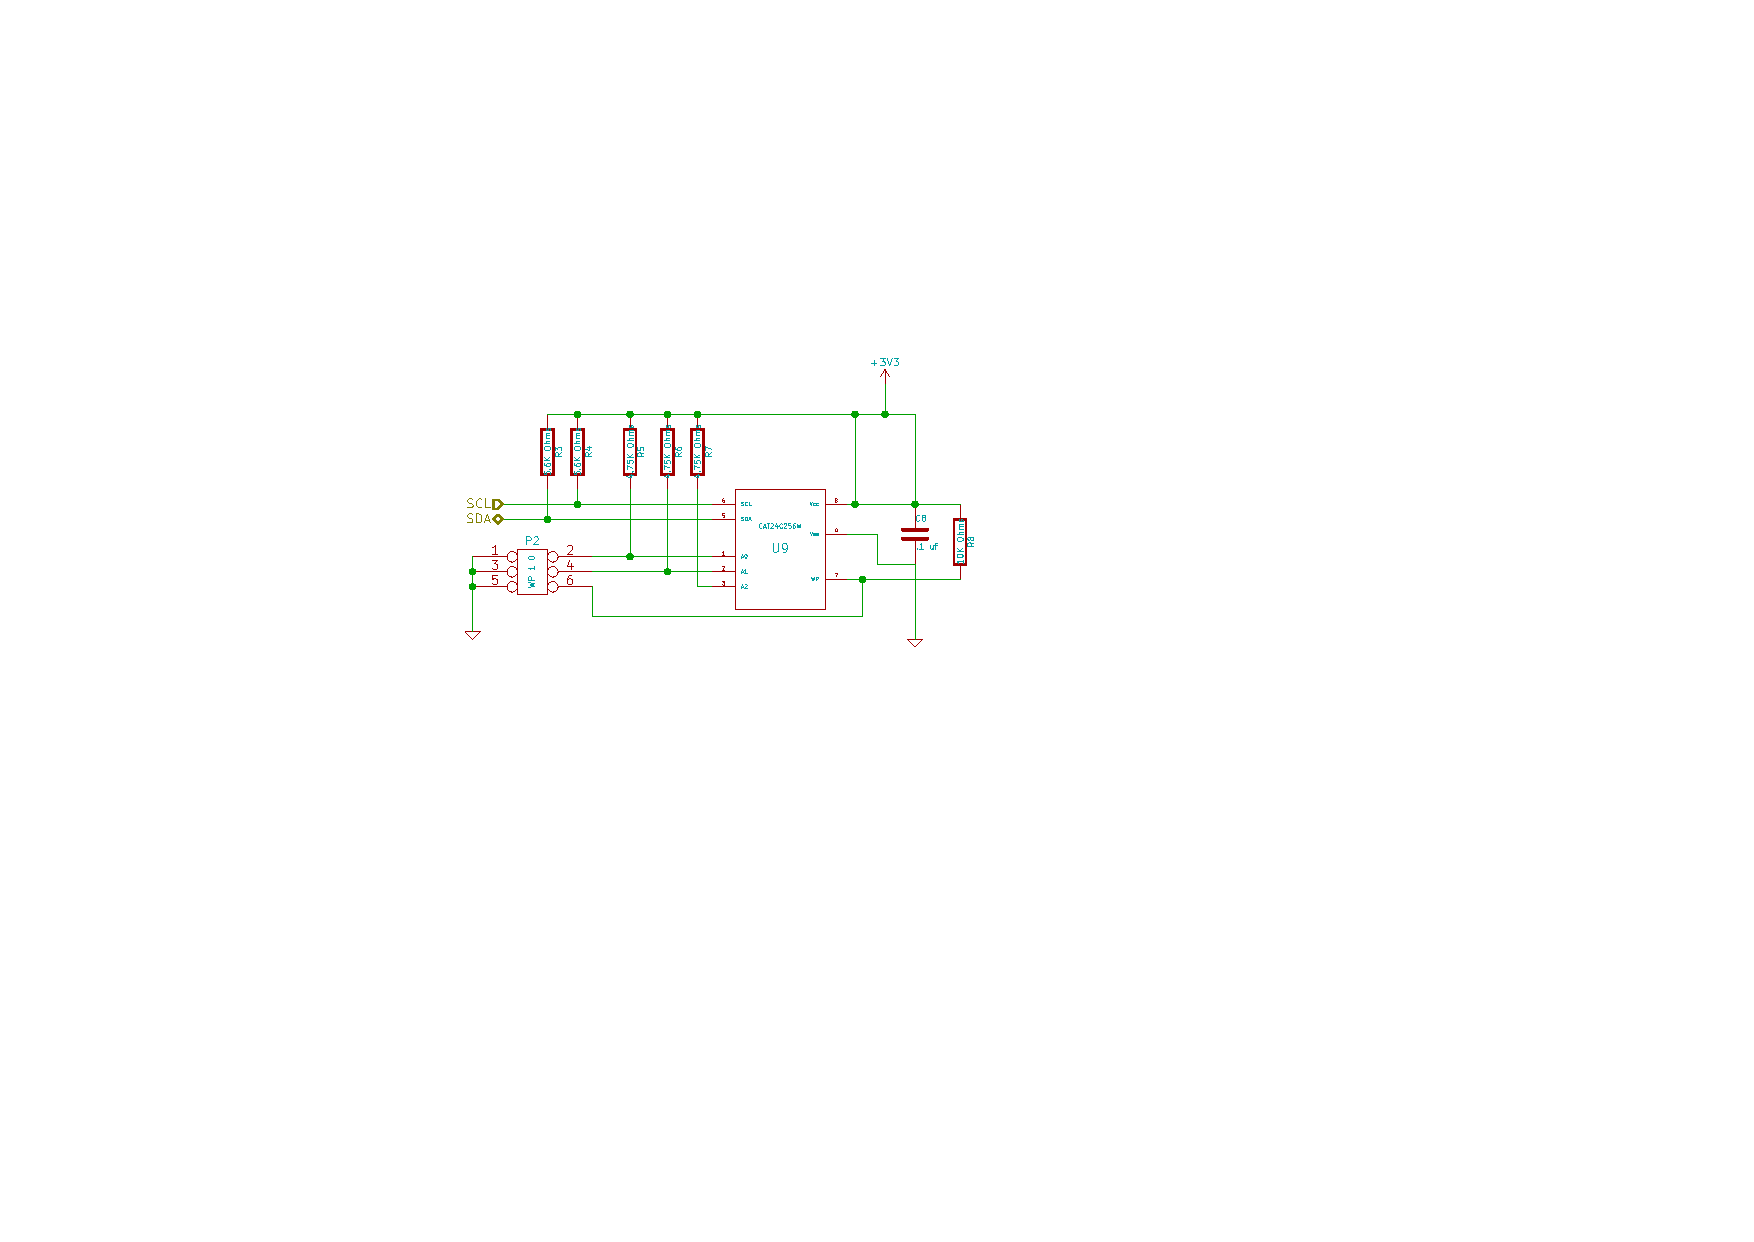
\includegraphics[width=5in]{QuadSMCSenseCape-2.pdf}
\caption{Circuit Diagram of the QuadSMCSenseCape, Sheet 2}
\end{centering}\end{figure}
This circuit contains three sections.  There is an output section that contains 
four TC4428 chips.  Each chip has a non-inverting and an inverting driver. The 
inputs of both drivers are connected to one of the motor GPIO pins.  The 
output are wired to the terminal block for a one of the motors. For any given 
logic state of the motor control output, one of the drivers is ``on'' and the 
other is ``off'', thus one motor terminal is ground and one is raised to the 
12V supply.  This means alternative states of the logic line will drive the 
stall motor in alternative directions.

The second section is a quartet of flip-flop debounce circuits, one for each
of two SPDT switch contacts that report the position of the turnout points.
The output of these flip-flops goes to a quartet of GPIO input pins.

The third section is the Cape EEProm circuit.  The Cape EEProm contains 
information about the cape and the name and version of the overlay that needs 
to be loaded by uBoot.

\section{Parts List}

\begin{table}[htdp]
\begin{centering}\begin{tabular}{|l|l|p{1in}|l|}
\hline
Value&Quantity&References&Mouser Part Number \\
\hline
10 uf 35V&1&''C1''&667-ECA-1HM100I \\
\hline
.1 uf&3&''C2 C3 C8''&581-SR201C104KARTR1 \\
\hline
WP 1 0&1&''P2''&649-67996-406HLF \\
\hline
BeagleBone\_Black\_Header&2&''P8 P9''&200-ESQ12314GD \\
\hline
4.75K Ohms&3&''R5 R6 R7''&603-CFR-25JR-524K7 \\
\hline 
5.6K Ohms&2&''R3 R4''&603-CFR-25JR-525K6 \\
\hline
10K Ohms&1&''R8''&603-CFR-25JR-5210K \\
\hline
10K Ohms&1&''RR1''&652-4609X-1LF-10K \\
\hline
Motor 1;Motor 2;Motor 3;Motor 4&4&T1 T2 T3 T4&651-1725685 \\
\hline
+ 12V -&1&''T5''&651-1725656 \\
\hline
TC4428&4&''U1 U2 U3 U4''&579-TC4428VPA \\
\hline
74HCT00&2&''U5 U6''&595-SN74AHC00N \\
\hline
CAT24C256W&1&''U9''&698-CAT24C256WI-GT3 \\
\hline
\end{tabular}
\caption{Parts list for QuadSMCSenseCape board.}
\end{centering}\end{table}\footnote{Mouser Project links: 
\url{http://www.mouser.com/ProjectManager/ProjectDetail.aspx?AccessID=330542c522},
\url{http://www.mouser.com/ProjectManager/ProjectDetail.aspx?AccessID=522a1259b2}.}


The only parts that might be substituted are P8 and P9 (the Beagle Bone Black
Headers), and T1 though T4 (the Motor terminals) and T5 (the 12 to 16 Volts
terminals). The parts listed are for the stacking headers for the Beagle Bone
Black Headers, and screw terminals for the Motor terminals and the motor power
terminals. Feel free to select a non-stacking header for the Beagle Bone Black
Headers and to select either pin arrays or spring terminals for the T1, T2,
T3, T4 and T5.

\section{Circuit Board Layout}

\begin{figure}[hbpt]\begin{centering}%
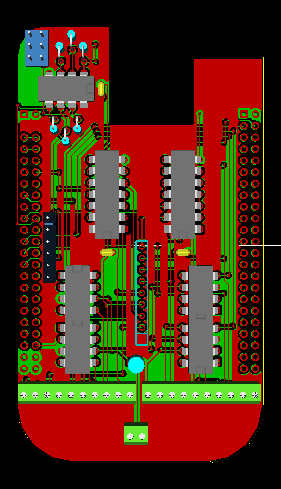
\includegraphics[height=7in]{QuadSMCSenseCape3DTop.png}
\caption{3D rendering of the QuadSMCSenseCape board}
\end{centering}\end{figure}
\begin{figure}[hbpt]\begin{centering}%
\includegraphics[height=7in]{QuadSMCSenseCape.png}
\caption{Fabrication image of the QuadSMCSenseCape board}
\end{centering}\end{figure}
Board assembly is straight forward. You need to be careful orienting the ICs
and the electrolytic capacitor.

Bare circuit boards can be ordered from PCBWay here: 
\url{https://www.pcbway.com/project/shareproject/Quad_Stall_motor_with_point_sense_cape.html}.

\section{Downloadables and Software Support}

Full design information is available on GitHub here:
\url{https://github.com/RobertPHeller/RPi-RRCircuits/tree/master/QuadSMCSenseCape}.

An OpenMRN program that supports this board is available here:
\url{https://github.com/RobertPHeller/RPi-RRCircuits/tree/master/QuadSMCSenseOpenMRN}.




